% Software Development for Mobile Devices
\documentclass[11pt,english,numbers=endperiod,parskip=half]{scrartcl}

\usepackage{color}
\usepackage{graphicx}
\usepackage{minted}
\usepackage{fancyhdr}
\usepackage{pdflscape}

\pagestyle{fancy}

\rhead{Daniel Parker - 971328X}
\lhead{COS30017 - Software Development for Mobile Devices}

\title{Assignment 05}
\subtitle{COS30017 - Software Development for Mobile Devices}
\author{Daniel Parker 971328X}

\date{\today}

\begin{document}
\maketitle
\thispagestyle{empty}

\section{Task 1}

\section{Task 2}
\subsection{User Stories}
\begin{enumerate}
	\item{As a recreational road-cyclist, I want to get the sun rise time and
	weather conditions so that I can maximise the time riding in daylight before
	I go to work.}
	\item{As an adventure tour guide, I want to know the sun set times for a
	period of a week so that my group of campers can have their tents set up
	before sundown.}
	\item{As a group runner, I want to be able to share the sun rise time with
	those that I'm running with so that we can all be ready to run as soon as
	there's daylight.}
	\item{As a zookeeper, I need to know the sun rise times so that I can plan
	to clean the animal enclosures and feed the animals before the zoo opens.}
\end{enumerate}
\subsection{User Stories vs. Scenarios}
When comparing user stories and scenarios as a way of showing how an application
 may be used, I think it user stories are better to use, due to the fact that
they are shorter and tend to only focus on one specific feature. The Scenarios
have a lot of information, and potentially every single feature can be listed as
 part of the scenario story. This leads tohaving to go thoroughly through the
scenarios to actually get the important information out.
\subsection{Prototype}
\subsubsection{Screenshots}
\setlength\fboxsep{0pt}
\setlength\fboxrule{0.5pt}

\begin{figure}[H]
\centering{
	\fbox{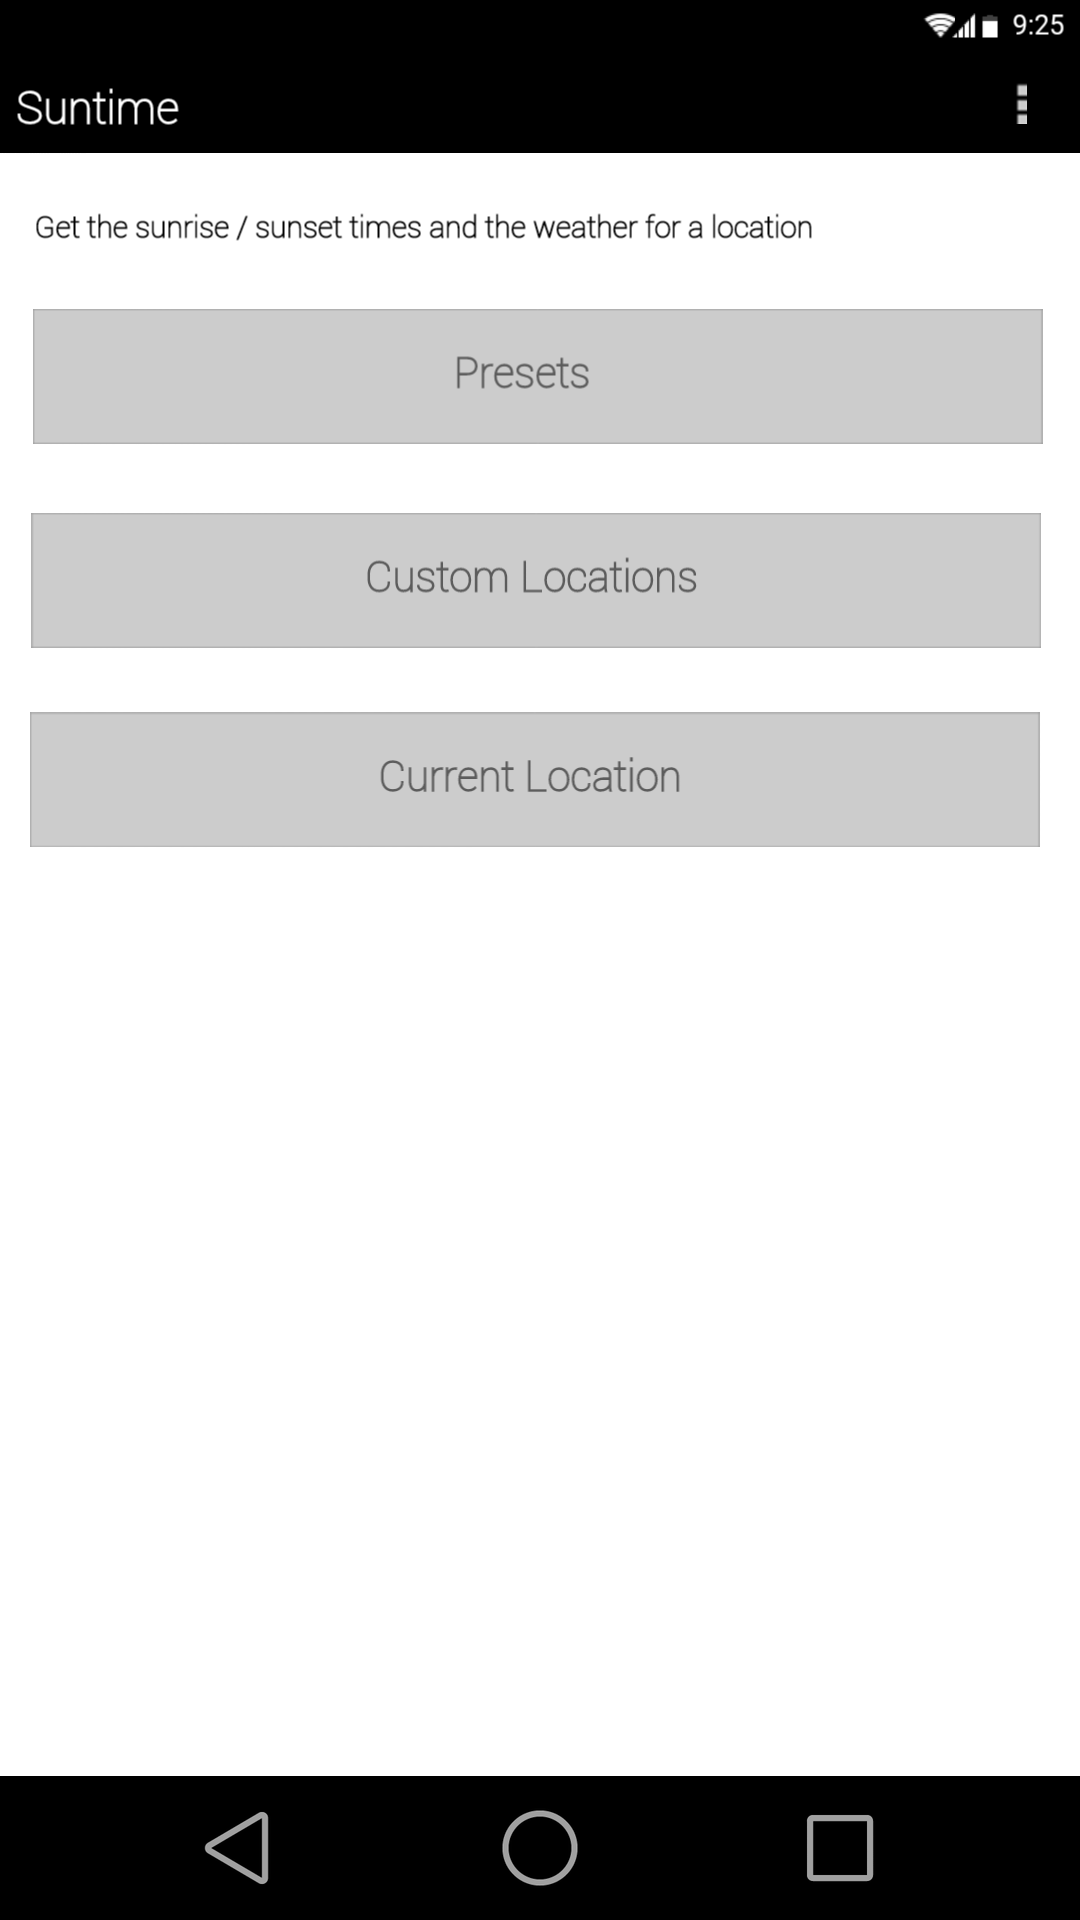
\includegraphics[width=5cm]{images/home.png}}
	\caption{HOME}
}
\end{figure}
\bigskip
\textbf{Description: }This is the first screen the user will see.
The user has three options for selecting a location;
\textit{Presets}, \textit{Custom Locations}, and \textit{Current Location}.

\textbf{Features: }Options for locations as described above. Can detect current
location as an option.

\begin{figure}[H]
\centering{
	\fbox{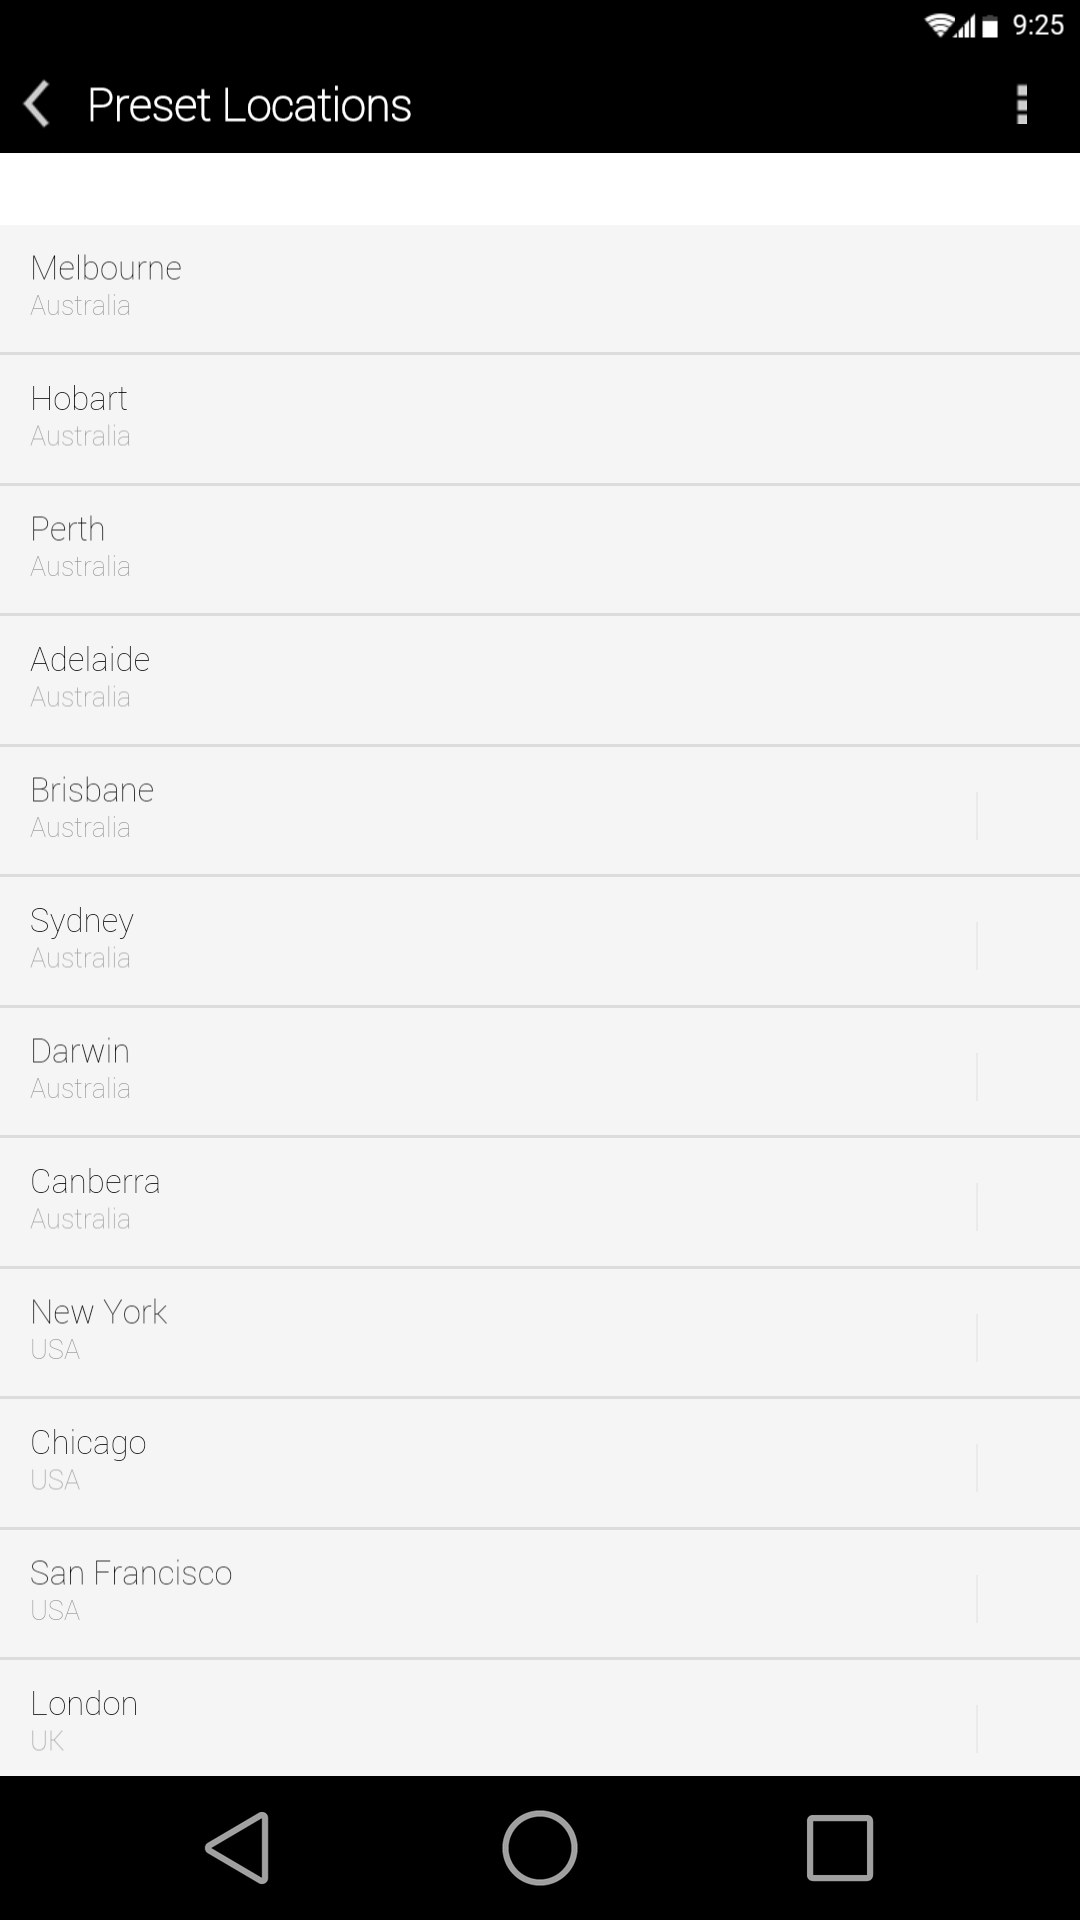
\includegraphics[width=5cm]{images/presets.png}}
	\caption{PRESETS}
}
\end{figure}
\bigskip
\textbf{Description: }The user can select one of the preset locations from this
list and they will then be taken to select a date / date range.

\textbf{Features: }Select from pre-built set of locations.

\begin{figure}[H]
\centering{
	\fbox{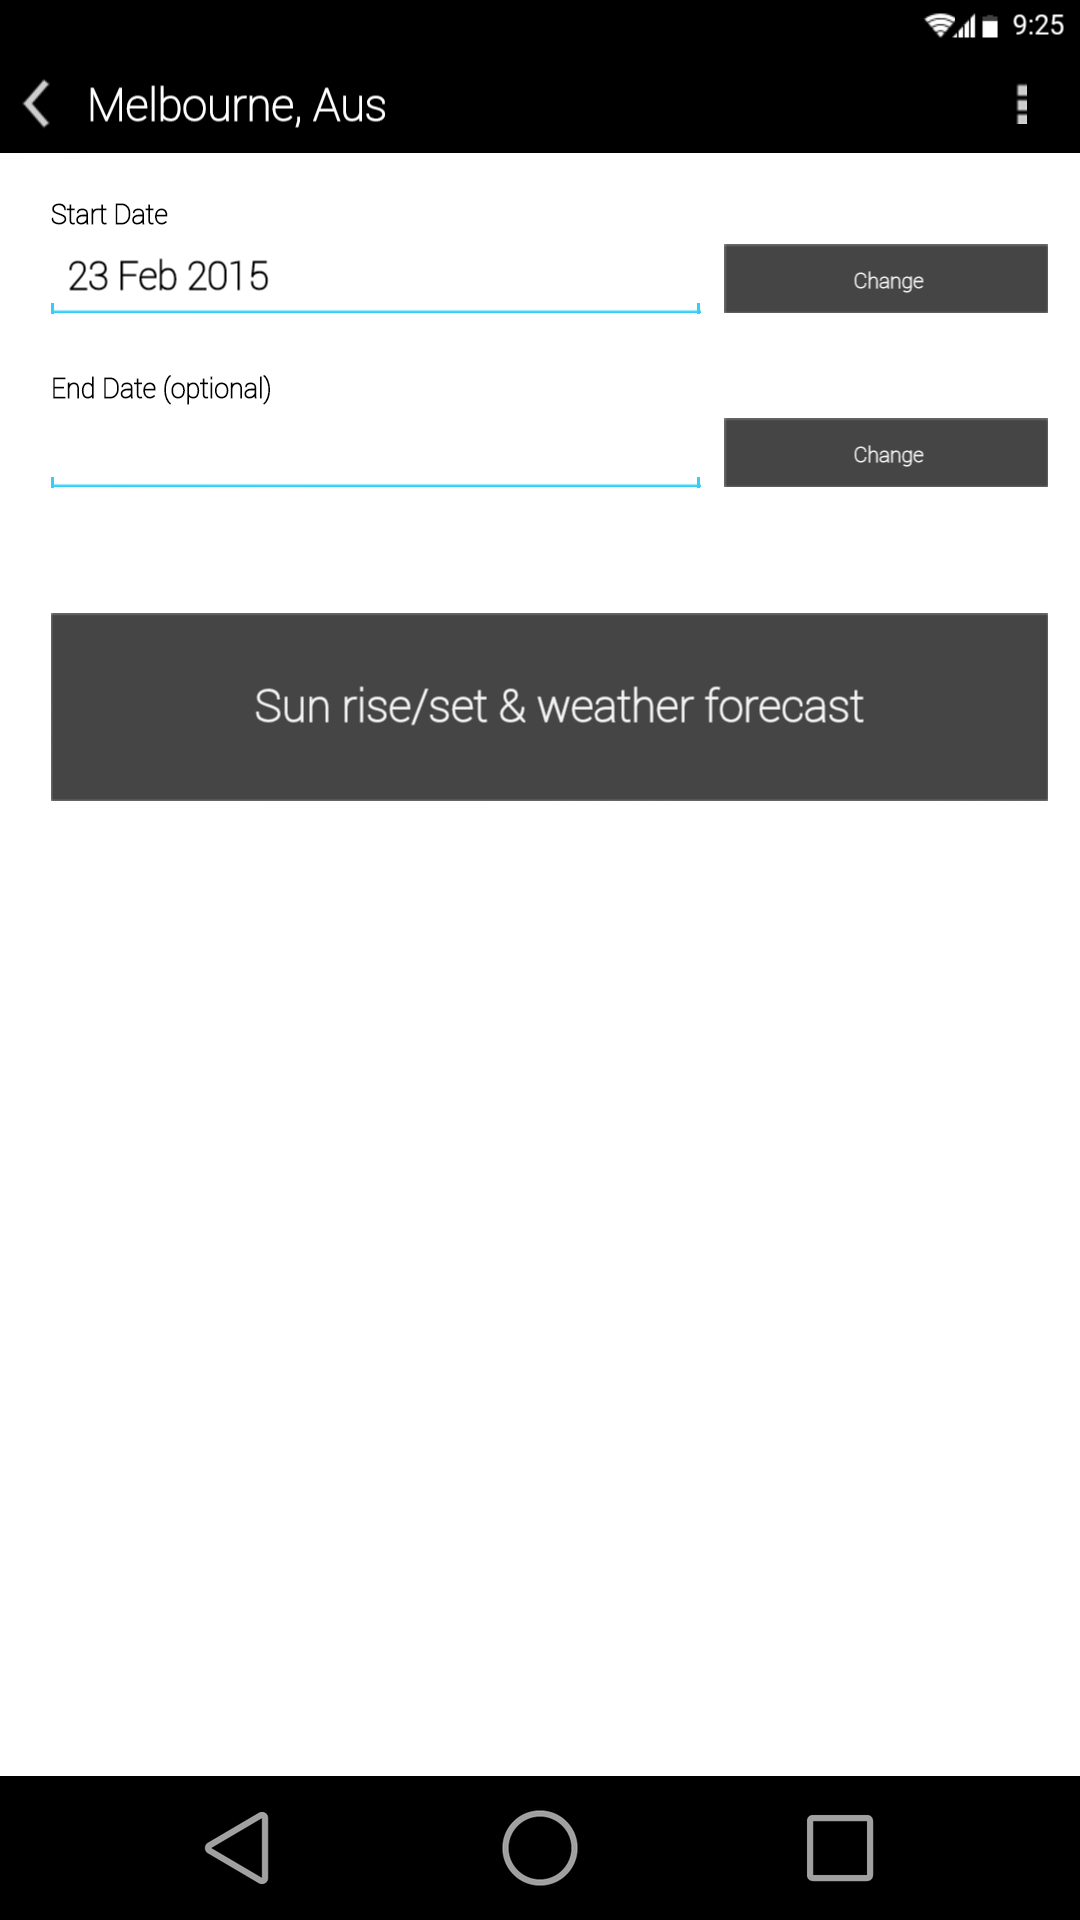
\includegraphics[width=5cm]{images/date-single.png}}
	\caption{DATE-SELECT}
}
\end{figure}
\bigskip
\textbf{Description: }User can select a single date or date range to view the
sun rise/set and weather. A different view is shown to them depending on whether
a single date or a range is selected.

\textbf{Features: }Select a date or a date range to view sun times and weather forecast.

\begin{figure}[H]
\centering{
	\fbox{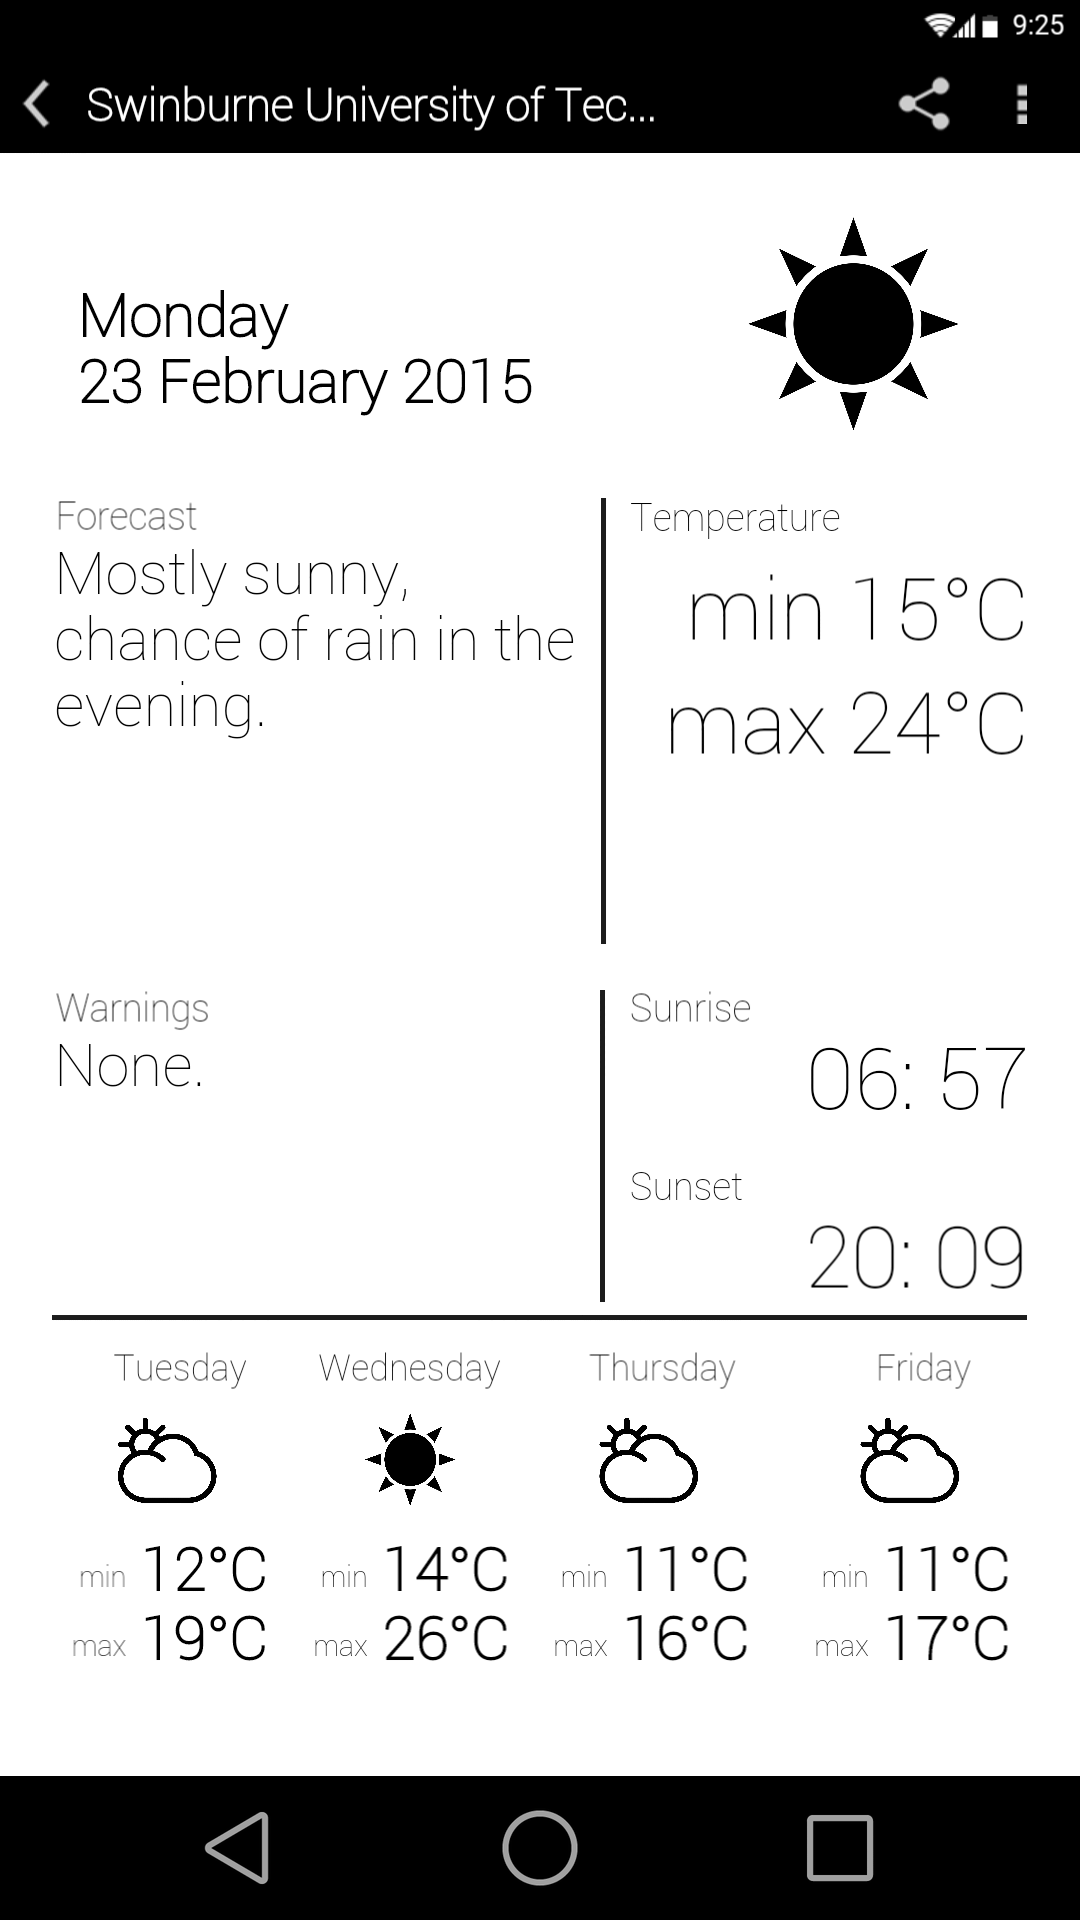
\includegraphics[width=5cm]{images/weather.png}}
	\caption{SUN-WEATHER}
}
\end{figure}
\bigskip
\textbf{Description: }This screen shows the weather and sun rise/set times for
the selected date. The weather for the next 4 days is also shown. User can share
this information by pressing the share icon in the action bar.

\textbf{Features: }Show sun rise/set times for date/location. Share information
via SMS and email (or any other app). View weather forecast (current, and near future).

\begin{figure}[H]
\centering{
	\fbox{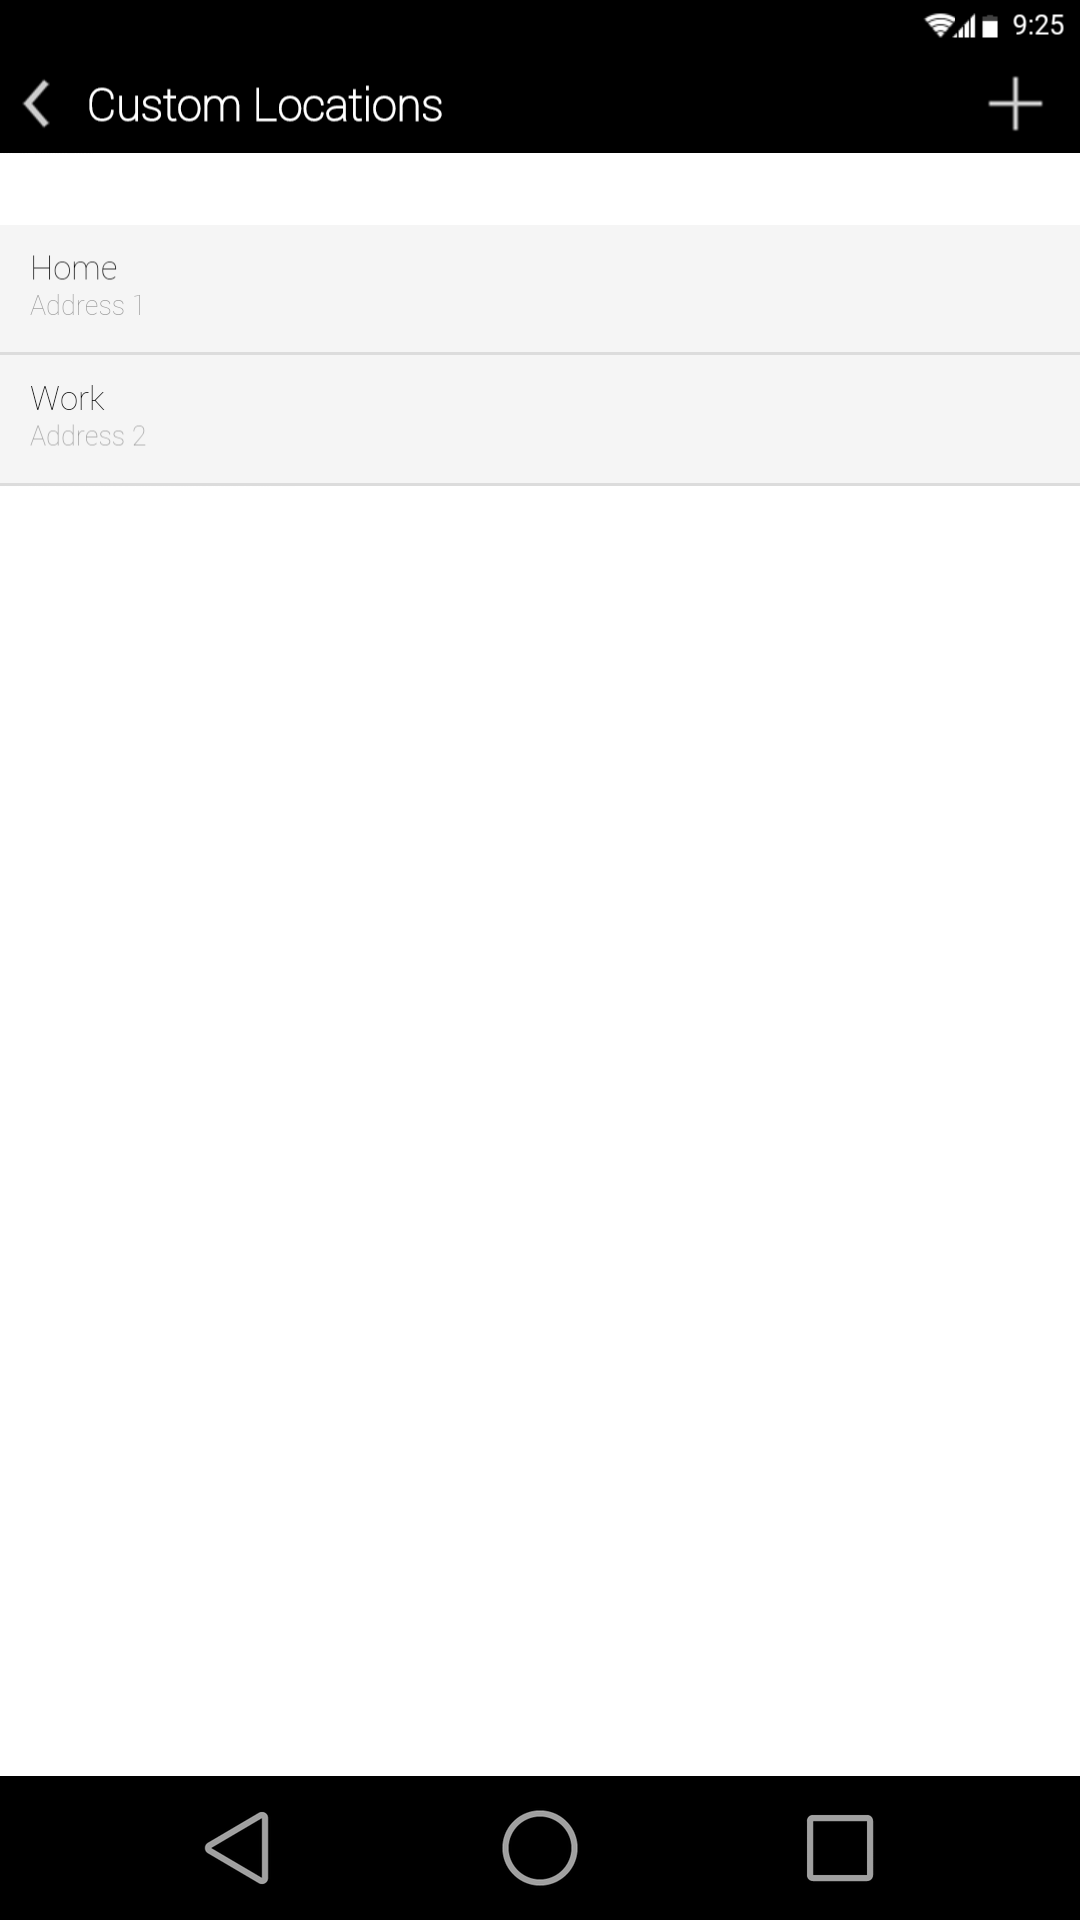
\includegraphics[width=5cm]{images/custom-list.png}}
	\caption{CUSTOM}
}
\end{figure}
\bigskip
\textbf{Description: }The user can select one of their previous custom locations
or press the \(+\) symbol to take them to add another custom location.

\textbf{Features: }Add new custom location (partial).

\begin{figure}[H]
\centering{
	\fbox{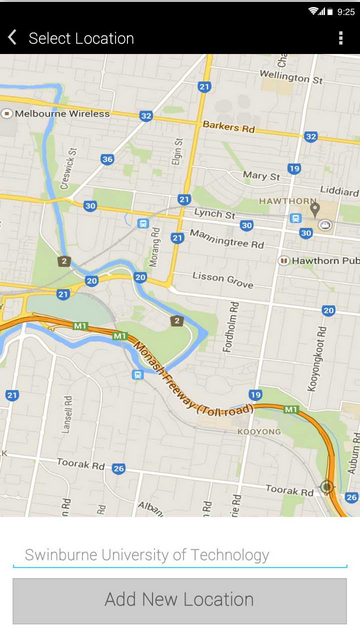
\includegraphics[width=5cm]{images/map.png}}
	\caption{MAP}
}
\end{figure}
\bigskip
\textbf{Description: }User can either pin a point on the map or search for a
location in the search bar. This will add it to the custom locations list and
allow them to see the sun times and weather.

\textbf{Features: }Add custom locations. Integrated into Google maps. View sun
rise / set times for various locations on a map.

\begin{figure}[H]
\centering{
	\fbox{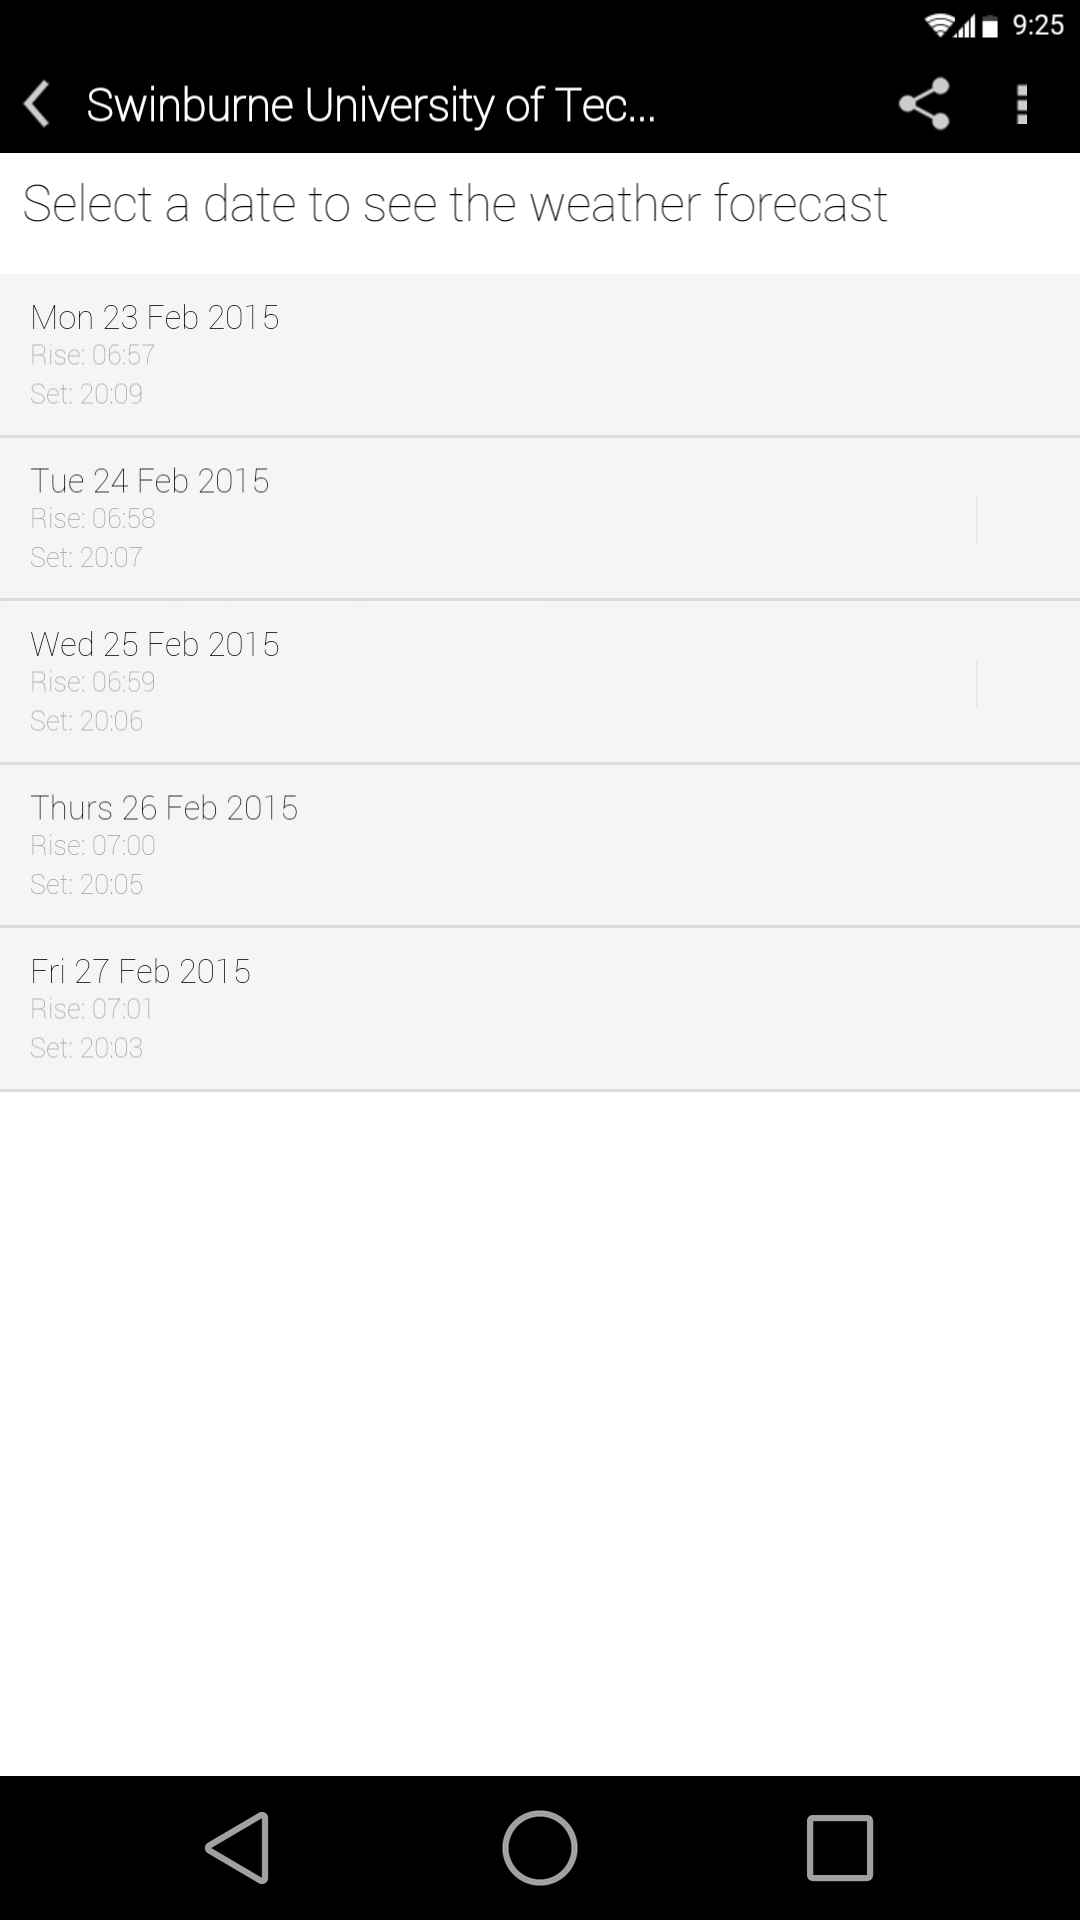
\includegraphics[width=5cm]{images/sun-range.png}}
	\caption{SUN-RANGE}
}
\end{figure}
\bigskip
\textbf{Description: }This screen shows the sun times for a range of dates which
was requested on the previous screen \textit{DATE-SELECT}. User can click on any
date and see the full \textit{WEATHER} screen as well.

\textbf{Features: }Generate table of sun rise/set times for a date range.
% \raggedright
% The Metadata app contains two activities. The main activity contains a listview of all the ImageData objects and the list item layout is specified in a separate xml layout file. The wiring of these two activities uses the parcelable protocol. The ImageData class implements the Parcelable interface as it is the data that will be sent between the two activities. The EditMetadata activity is called using StartActivityForResult because the edited ImageData object needs to be returned and the updated metadata shown in the listview. The label text sizes are set using styles. The user can change the size of the text by selecting a different option from the dropdown list in the EditMetadata activity, which changes the theme of the activity and subsequently the text size for the labels.
% \subsection{What is the Parcelable protocol}
% \raggedright
% The Parcelable protocol is a method for serializing object data so that it can be sent between activities as context. In the case of this Metadata app, when a user selects an image to edit, the underlying ImageData object is serialized as per the Parcelable interface implementation and sent to the EditMetadata activity. That activity will deserialize the object from using the parcelable interface so that it can be accessed like a normal object and edited. The same is done when the object is returned as a result from the EditMetadata activity. The reason we do not use the Serializable interface is that the Parcelable interface is significantly quicker to serialize and deserialize. This is desirable for Android apps considering that they run on lower powered devices and time is critical with these simple user interface wiring tasks.
%
% \subsection{screenshots}
% \setlength\fboxsep{0pt}
% \setlength\fboxrule{0.5pt}
%

% \centering{
% 	\fbox{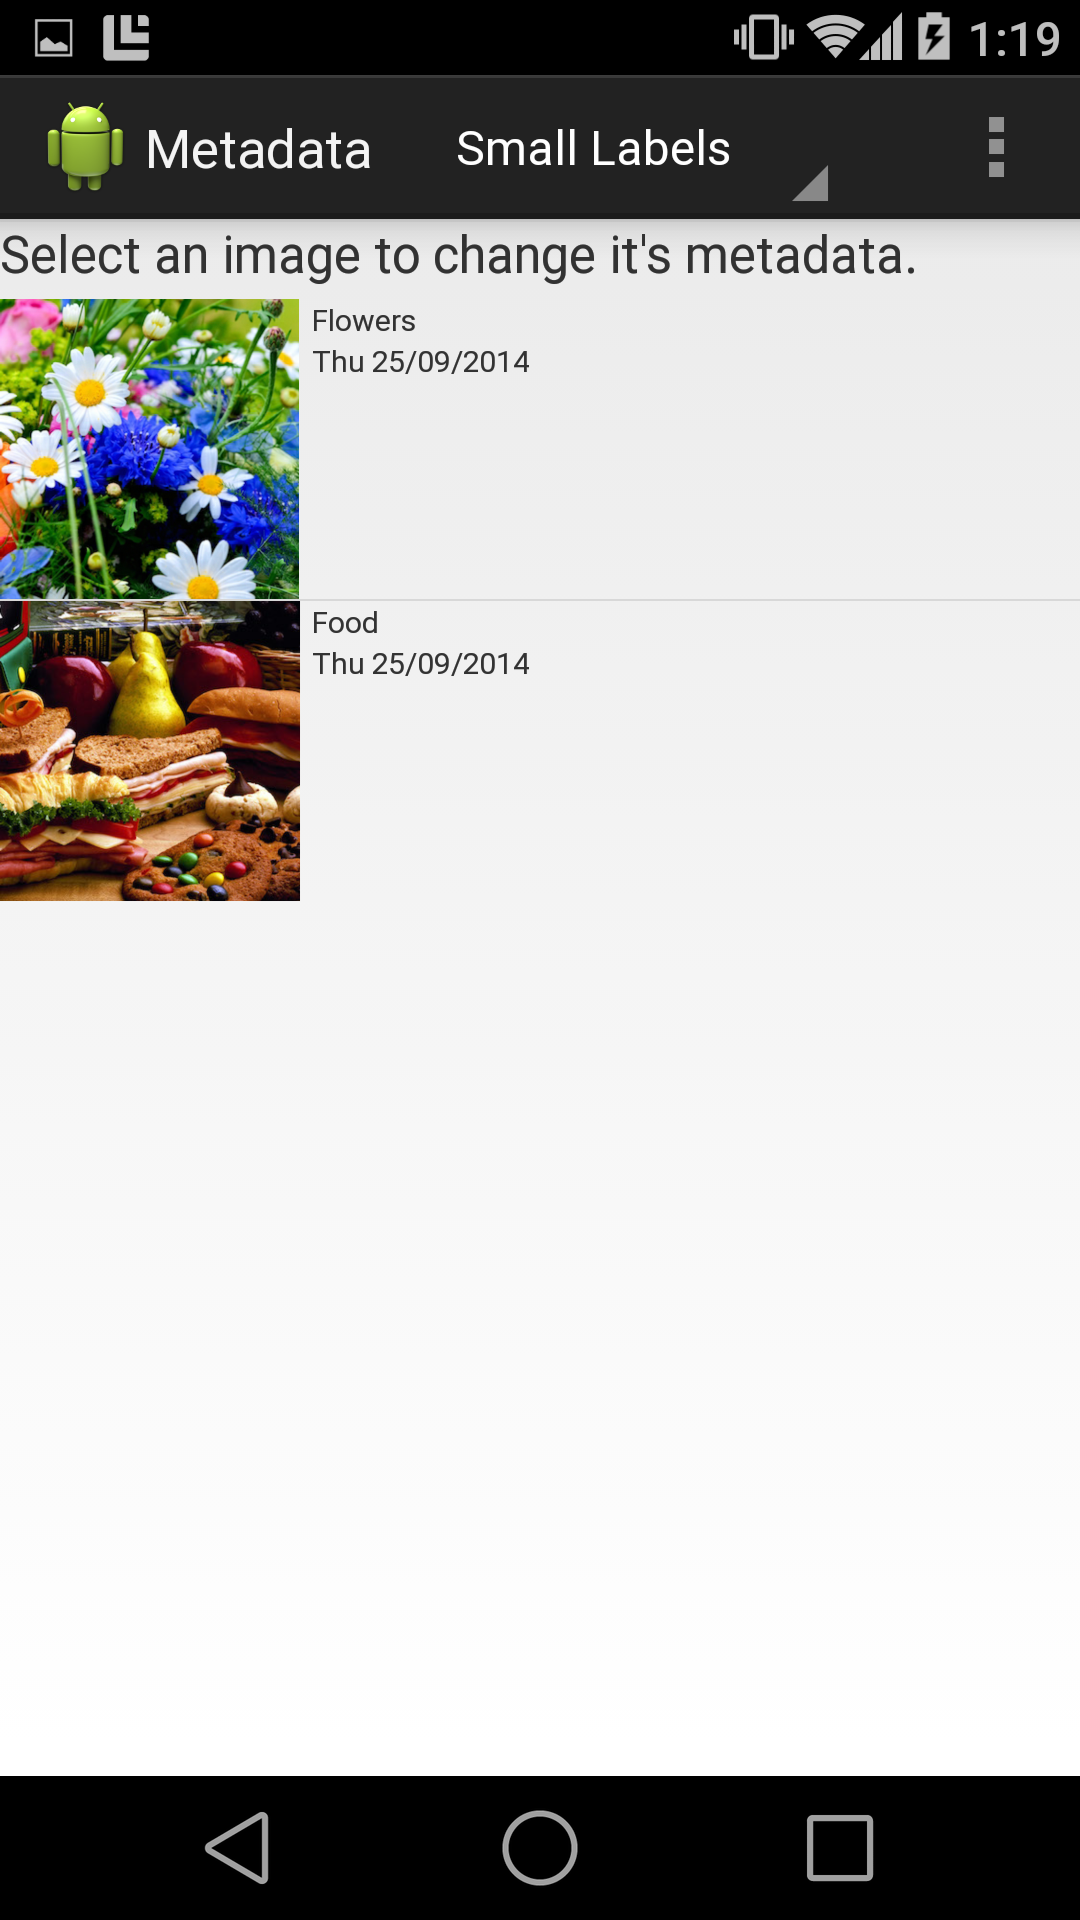
\includegraphics[width=5cm]{images/home-s.png}}
% }\\
% \bigskip
% \centering{
% 	\fbox{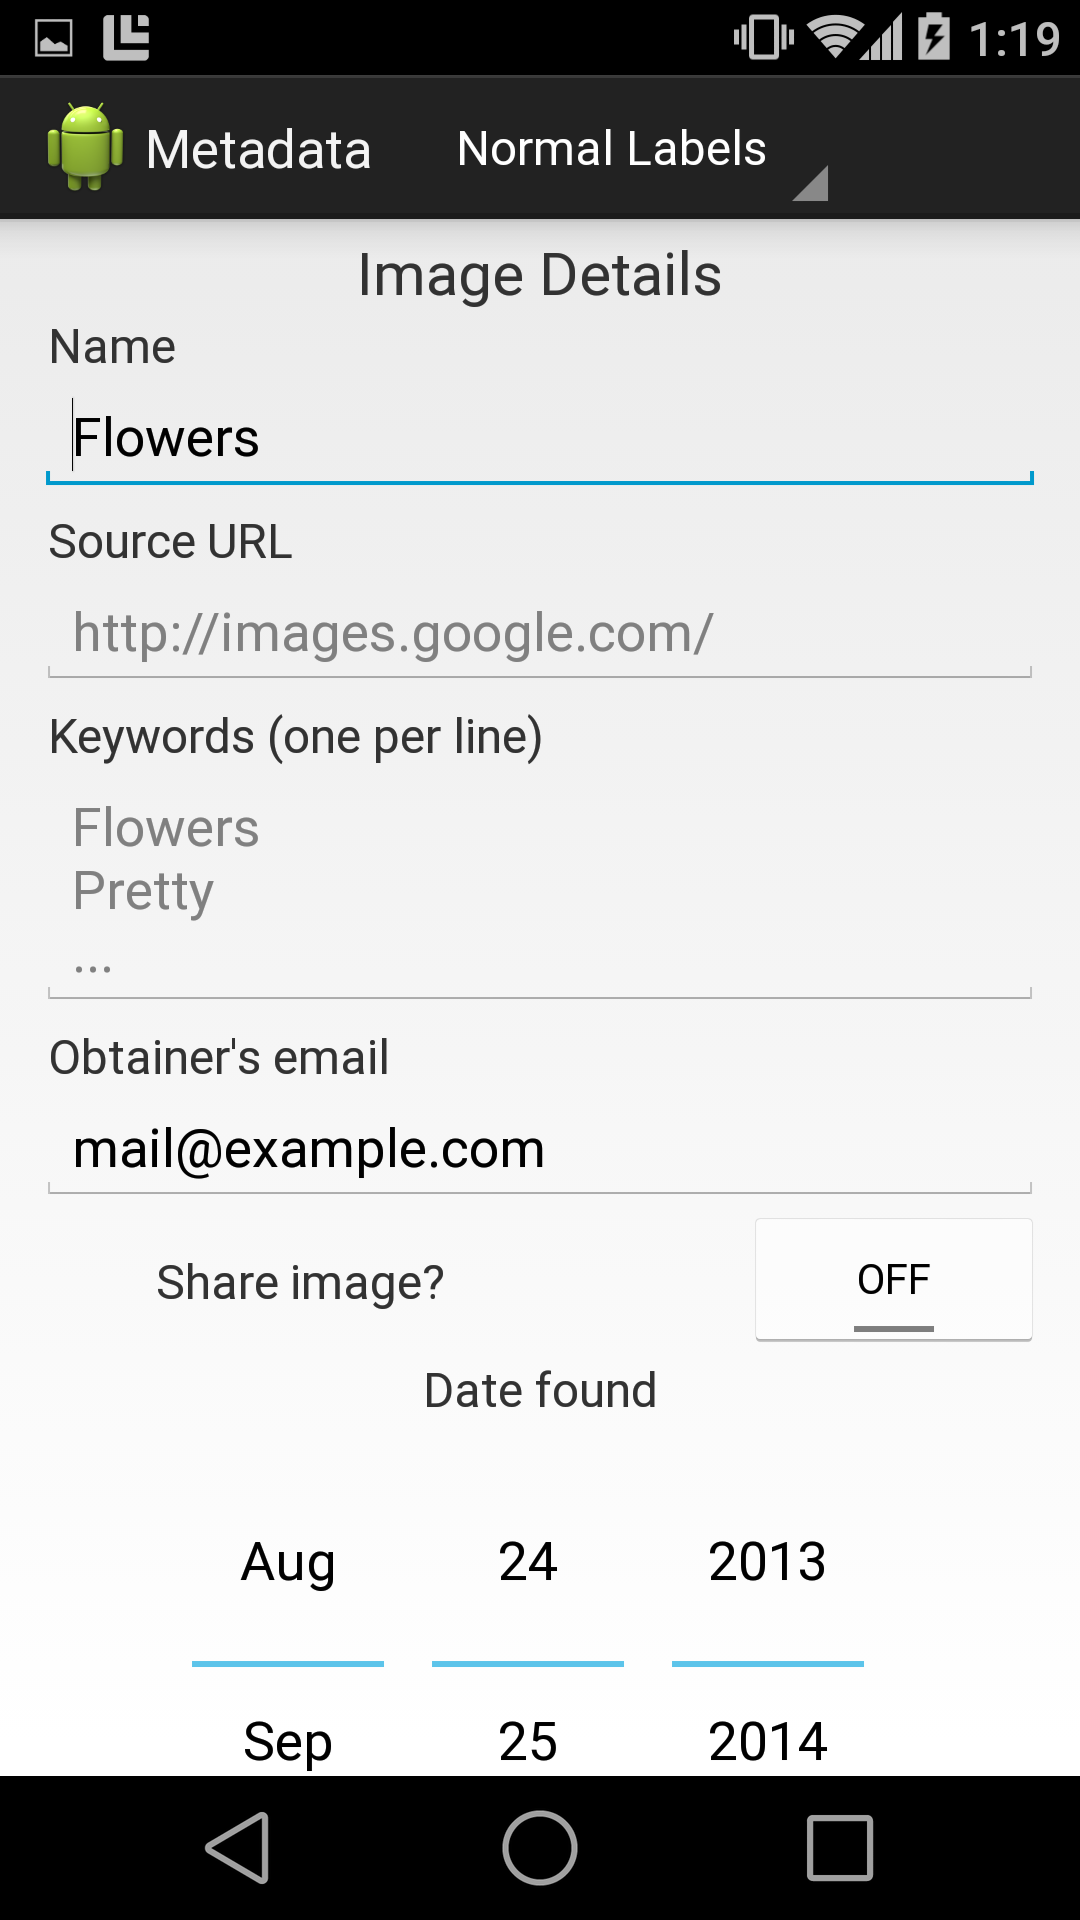
\includegraphics[width=5cm]{images/meta-n.png}}
% }\\
% \bigskip
% \centering{
% 	\fbox{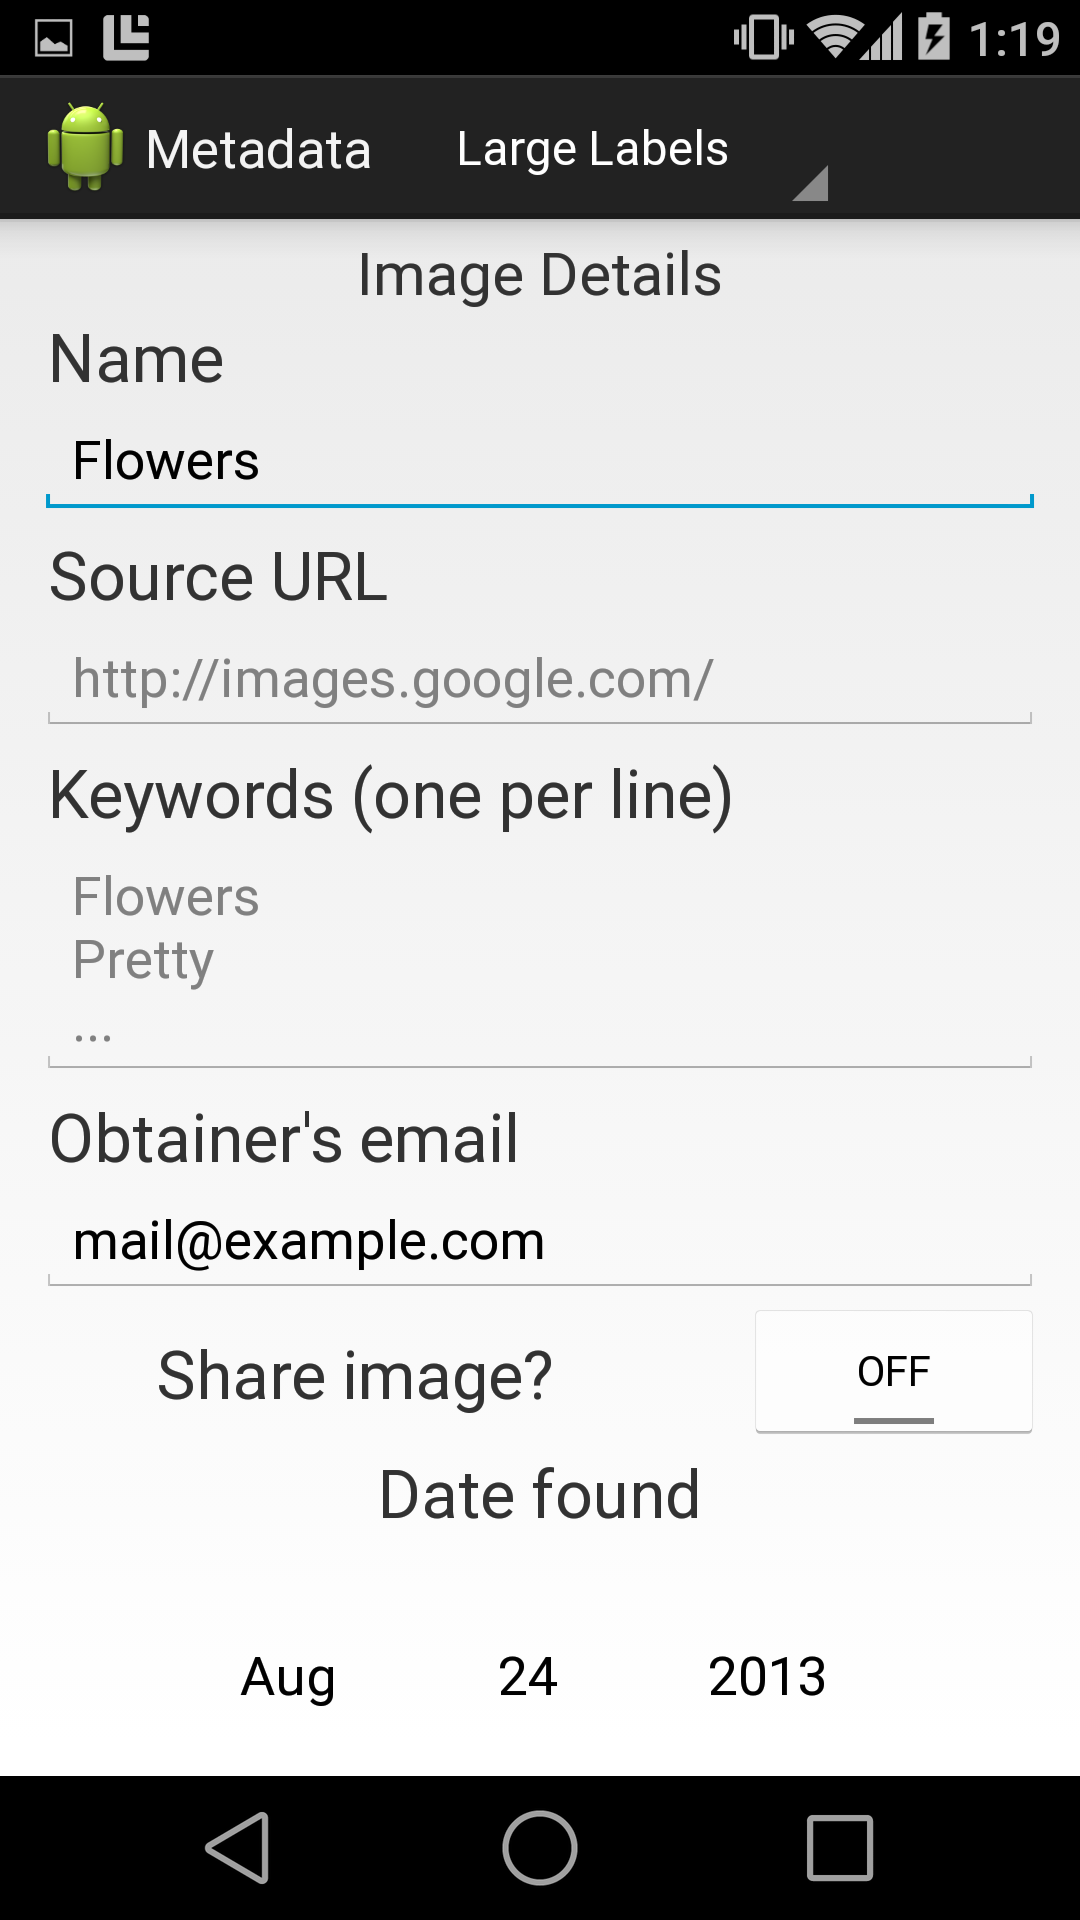
\includegraphics[width=5cm]{images/meta-l.png}}
% }\\
% \bigskip
% \centering{
% 	\fbox{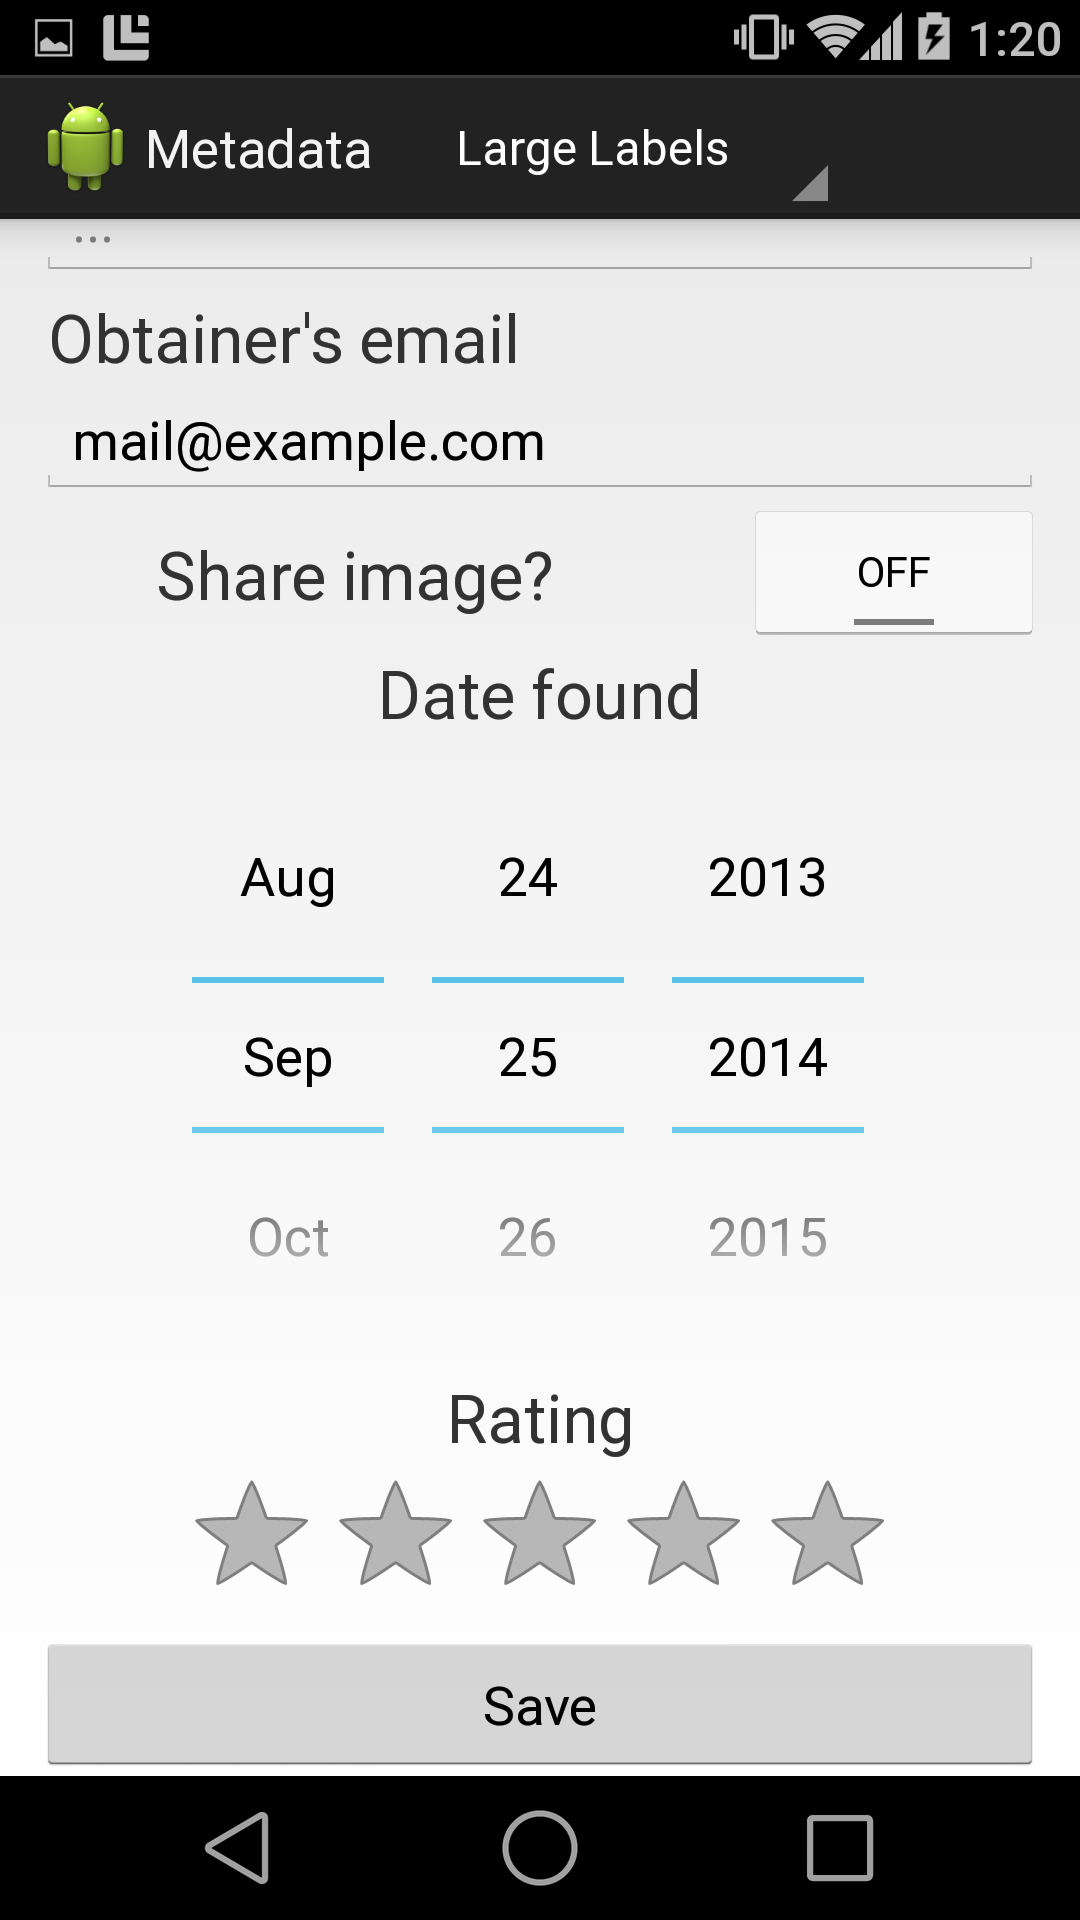
\includegraphics[width=5cm]{images/meta-l-bottom.png}}
% }\\
% \bigskip
%
%
% \begin{landscape}
% \subsection{Source}
% \subsubsection{Gallery.java (Startup activity)}
% \inputminted{java}{../../Apps/Metadata/app/src/main/java/au/net/danielparker/metadata/Gallery.java}
%
% \subsubsection{EditMetadata.java}
% \inputminted{java}{../../Apps/Metadata/app/src/main/java/au/net/danielparker/metadata/EditMetadata.java}
%
% \subsubsection{ImageData.java}
% \inputminted{java}{../../Apps/Metadata/app/src/main/java/au/net/danielparker/metadata/ImageData.java}
%
% \subsubsection{activity\_gallery.xml}
% \inputminted{xml}{../../Apps/Metadata/app/src/main/res/layout/activity_gallery.xml}
%
% \subsubsection{gallery\_item.xml}
% \inputminted{xml}{../../Apps/Metadata/app/src/main/res/layout/gallery_item.xml}
%
% \subsubsection{activity\_edit\_metadata.xml}
% \inputminted{xml}{../../Apps/Metadata/app/src/main/res/layout/activity_edit_metadata.xml}
%
% \subsubsection{styles.xml}
% \inputminted{xml}{../../Apps/Metadata/app/src/main/res/values/styles.xml}
% \end{landscape}
%
% \section{Usability Test}
% \subsection{Objective}
% \raggedright
% The purpose of this usability test was to identify what label font size felt most comfortable visually for users and also what information display font size was the best. It isn't always obvious what users will prefer, but doing a usability test like this one can help to identify the best font size for the situation.
% \subsection{Method}
% \begin{enumerate}
% 	\item{The three font sizes were selected by first selecting a font size that looked best in my own opinion. That value was then used as the middle font size and font sizes slightly smaller and larger were selected as the other two font sizes for the usability test.}
% 	\item{The three selected font sizes were:
% 		\begin{itemize}
% 			\item{Small: 10sp}
% 			\item{Medium: 16sp}
% 			\item{Large: 22sp}
% 		\end{itemize}
% 	}
% 	\item{The code used three different themes to change the font size. The three themes simple overrode the android value for labelTextSize, which was referenced as the text size for labels using the attribute \textit{android:textSize="?android:attr/labelTextSize"}. The user can then select the size they want within the EditMetadata activity and the theme will be set and activity reloaded.}
% \end{enumerate}
% \subsection{Participants}
% \begin{enumerate}
% 	\item{
% 			\begin{itemize}
% 				\item{Age: 55}
% 				\item{Occupation: Personal Assistant}
% 				\item{Computer usage: Daily}
% 				\item{Smartphone: Owns a smartphone}
% 			\end{itemize}
% 		}
% 	\item{
% 			\begin{itemize}
% 				\item{Age: 56}
% 				\item{Occupation: Software Engineer}
% 				\item{Computer usage: Daily}
% 				\item{Smartphone: Does not own a smartphone}
% 			\end{itemize}
% 		}
% 	\item{
% 			\begin{itemize}
% 				\item{Age: 24}
% 				\item{Occupation: Waitress}
% 				\item{Computer usage: Once a month}
% 				\item{Smartphone: Owns a smartphone}
% 			\end{itemize}
% 		}
% \end{enumerate}
% \subsection{Results}
% \subsubsection{Participant 1}
% \begin{table}[H]
% 	\begin{tabular}{| p{0.55\linewidth} | p{0.15\linewidth} | p{0.15\linewidth} | p{0.15 \linewidth} |}
% 		\hline
% 			&	Small	&	Medium	&	Large \\ \hline
% 		Can you read the text?	& Only Just	& Yes	& Yes \\ \hline
% 		Do you prefer this font size for the labels? & No & Yes & No \\ \hline
% 		Do you prefer this font size for the information display? & No & Yes & No \\
% 		\hline
% 	\end{tabular}
% \end{table}
%
% \subsubsection{Participant 2}
% \begin{table}[H]
% 	\begin{tabular}{| p{0.55\linewidth} | p{0.15\linewidth} | p{0.15\linewidth} | p{0.15 \linewidth} |}
% 		\hline
% 			&	Small	&	Medium	&	Large \\ \hline
% 		Can you read the text?	& No & Yes	& Yes \\ \hline
% 		Do you prefer this font size for the labels? & No & Yes & No \\ \hline
% 		Do you prefer this font size for the information display? & No & Yes & Yes \\
% 		\hline
% 	\end{tabular}
% \end{table}
%
% \subsubsection{Participant 3}
% \begin{table}[H]
% 	\begin{tabular}{| p{0.55\linewidth} | p{0.15\linewidth} | p{0.15\linewidth} | p{0.15 \linewidth} |}
% 		\hline
% 			&	Small	&	Medium	&	Large \\ \hline
% 		Can you read the text?	& Yes	& Yes	& Yes \\ \hline
% 		Do you prefer this font size for the labels? & No & Yes & No \\ \hline
% 		Do you prefer this font size for the information display? & No & Yes & No \\
% 		\hline
% 	\end{tabular}
% \end{table}
%
% \subsection{Recommendation}
% \raggedright
% The recommendation from the results of the usability test is that the Medium 16sp font size is used for labels and information display. This is due to all of the tested users saying that they could read and preferred that size for the label and display information text.
%
% \subsection{Reflection}
% \raggedright
% If the usability test were to be run again, the users would be show all the fonts first and then asked to only give one preferred out of the three fonts for the labels and display information.

\end{document}
